\begin{figure}[p]
\centering
    \begin{subfigure}[t]{0.45\textwidth}
    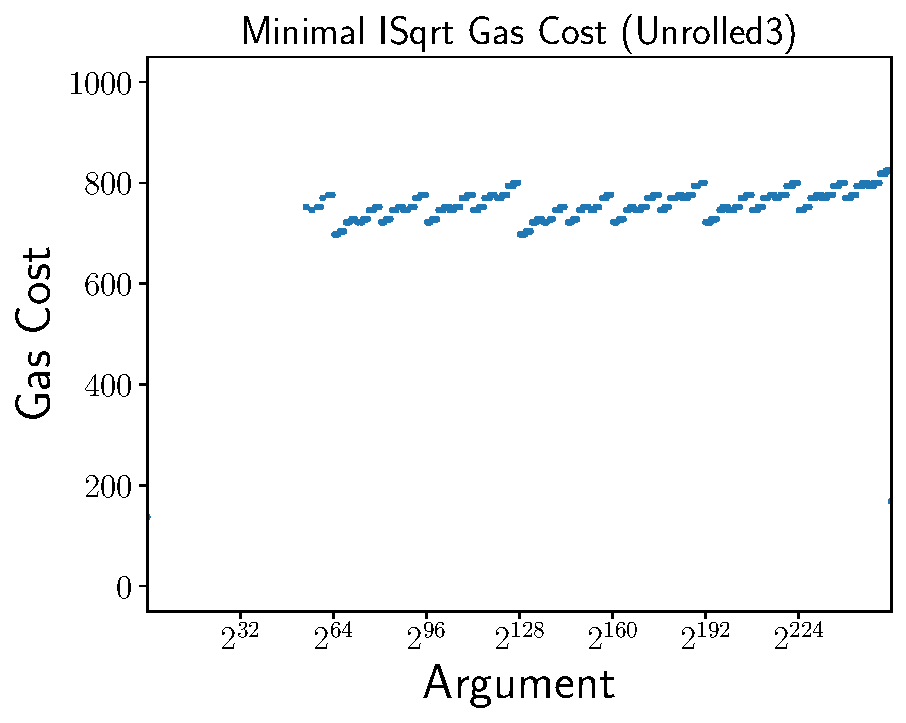
\includegraphics[width=\textwidth]{plots/minimal_plot_Unrolled3.pdf}
    \end{subfigure}
    \begin{subfigure}[t]{0.45\textwidth}
    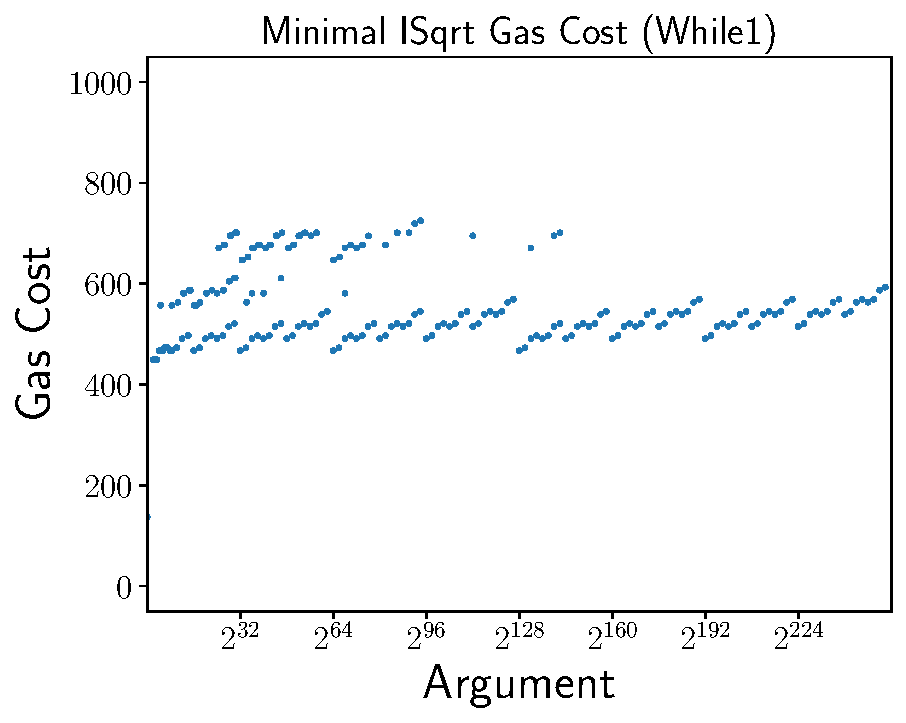
\includegraphics[width=\textwidth]{plots/minimal_plot_While1.pdf}
    \end{subfigure}

    \begin{subfigure}[t]{0.45\textwidth}
    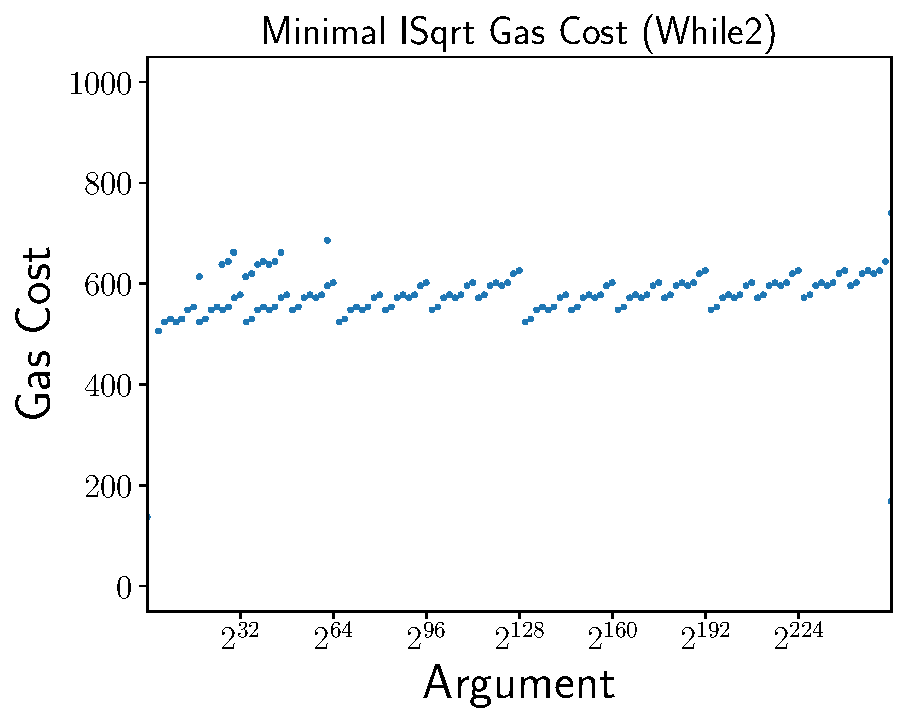
\includegraphics[width=\textwidth]{plots/minimal_plot_While2.pdf}
    \end{subfigure}
    \begin{subfigure}[t]{0.45\textwidth}
    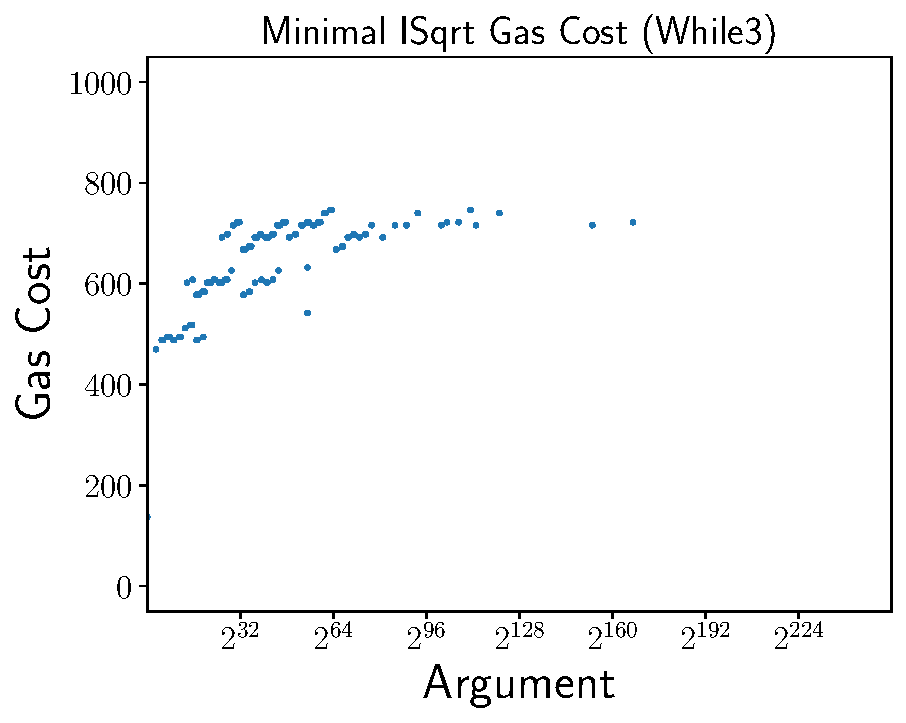
\includegraphics[width=\textwidth]{plots/minimal_plot_While3.pdf}
    \end{subfigure}
    \caption{Here we plot the instances where each algorithm is minimal.
        A histogram of this data may be found in
        Figure~\ref{fig:minimal_gas_hist}.
        These results are the for the tests in Section~\ref{sec:comparison}.
        }
    \label{fig:minimal_gas}
\end{figure}
